\documentclass[]{article}
\usepackage[T1]{fontenc}
\usepackage{lmodern}
\usepackage{amssymb,amsmath}
\usepackage{ifxetex,ifluatex}
\usepackage{fixltx2e} % provides \textsubscript
% Set line spacing
% use upquote if available, for straight quotes in verbatim environments
\IfFileExists{upquote.sty}{\usepackage{upquote}}{}
\ifnum 0\ifxetex 1\fi\ifluatex 1\fi=0 % if pdftex
  \usepackage[utf8]{inputenc}
\else % if luatex or xelatex
  \ifxetex
    \usepackage{mathspec}
    \usepackage{xltxtra,xunicode}
  \else
    \usepackage{fontspec}
  \fi
  \defaultfontfeatures{Mapping=tex-text,Scale=MatchLowercase}
  \newcommand{\euro}{€}
\fi
% use microtype if available
\IfFileExists{microtype.sty}{\usepackage{microtype}}{}
\usepackage[margin=1in]{geometry}
\usepackage{longtable,booktabs}
\usepackage{graphicx}
% Redefine \includegraphics so that, unless explicit options are
% given, the image width will not exceed the width of the page.
% Images get their normal width if they fit onto the page, but
% are scaled down if they would overflow the margins.
\makeatletter
\def\ScaleIfNeeded{%
  \ifdim\Gin@nat@width>\linewidth
    \linewidth
  \else
    \Gin@nat@width
  \fi
}
\makeatother
\let\Oldincludegraphics\includegraphics
{%
 \catcode`\@=11\relax%
 \gdef\includegraphics{\@ifnextchar[{\Oldincludegraphics}{\Oldincludegraphics[width=\ScaleIfNeeded]}}%
}%
\ifxetex
  \usepackage[setpagesize=false, % page size defined by xetex
              unicode=false, % unicode breaks when used with xetex
              xetex]{hyperref}
\else
  \usepackage[unicode=true]{hyperref}
\fi
\hypersetup{breaklinks=true,
            bookmarks=true,
            pdfauthor={Heather E. Wheeler1, Nicholas Knoblauch2, GTEx Consortium, Nancy J. Cox3, Dan L. Nicolae1, Hae Kyung Im1},
            pdftitle={Genetic architecture of transcriptome regulation and orthogonal tissue decompositon},
            colorlinks=true,
            citecolor=blue,
            urlcolor=blue,
            linkcolor=magenta,
            pdfborder={0 0 0}}
\urlstyle{same}  % don't use monospace font for urls
\setlength{\parindent}{0pt}
\setlength{\parskip}{6pt plus 2pt minus 1pt}
\setlength{\emergencystretch}{3em}  % prevent overfull lines
\setcounter{secnumdepth}{0}

%%% Change title format to be more compact
\usepackage{titling}
\setlength{\droptitle}{-2em}
  \title{Genetic architecture of transcriptome regulation and orthogonal tissue
decompositon}
  \pretitle{\vspace{\droptitle}\centering\huge}
  \posttitle{\par}
  \author{Heather E. Wheeler\textsuperscript{1}, Nicholas
Knoblauch\textsuperscript{2}, GTEx Consortium, Nancy J.
Cox\textsuperscript{3}, Dan L. Nicolae\textsuperscript{1}, Hae Kyung
Im\textsuperscript{1}}
  \preauthor{\centering\large\emph}
  \postauthor{\par}
  \predate{\centering\large\emph}
  \postdate{\par}
  \date{2015-05-19 16:14:53 \textsuperscript{1}Department of Medicine,
University of Chicago, \textsuperscript{2}Committee on Genetics,
Genomics, and Systems Biology, University of Chicago,
\textsuperscript{3}Division of Genetic Medicine, Vanderbilt University}




\begin{document}

\maketitle


\section{Abstract}\label{abstract}

\emph{Lorem ipsum dolor sit amet, est ad doctus eligendi scriptorem. Mel
erat falli ut. Feugiat legendos adipisci vix at, usu at laoreet
argumentum suscipiantur. An eos adhuc aliquip scriptorem, te adhuc dolor
liberavisse sea. Ponderum vivendum te nec, id agam brute disputando
mei.}

\section{Introduction}\label{introduction}

Lorem ipsum dolor sit amet, est ad doctus eligendi scriptorem. Mel erat
falli ut. Feugiat legendos adipisci vix at, usu at laoreet argumentum
suscipiantur. An eos adhuc aliquip scriptorem, te adhuc dolor
liberavisse sea. Ponderum vivendum te nec, id agam brute disputando mei.

Putant numquam tacimates at eum. Aliquip torquatos ex vis, mei et quando
debitis appareat, impetus accumsan corrumpit in usu. Nam mucius facilis
singulis id, duo ei autem imperdiet instructior. Cu ceteros alienum mel,
id vix putant impedit, ex idque eruditi forensibus eum. Posse dicunt id
usu. Ei iracundia constituto sed, duo ne exerci ignota, an eum unum
conceptam.

Has audire salutandi no, ut eam dicat libris dicunt. Pri hendrerit
quaerendum adversarium ea, dicat atqui munere et sea. Illum insolens eos
ne, eu enim graece rationibus mea. At postea utamur mel, eius nonumes
percipitur at vis. Numquam similique in per, te quo saepe utroque
pericula.

Ea nonumy volumus usu, no mel inermis dissentias. Dico partiendo
vituperatoribus eum et. Mea accusam convenire te, usu populo qualisque
gloriatur ut. Eu eum oratio altera option, ad mea ignota scriptorem. Ne
suas latine vix, eos oblique sanctus pertinax cu.

\section{Results}\label{results}

\subsection{Local genetic variation explains a large proportion of gene
expression
variance}\label{local-genetic-variation-explains-a-large-proportion-of-gene-expression-variance}

We estimated the heritability of gene expression in whole blood from the
Depression Genes and Networks (DGN) cohort (n=922) {[}1{]} using a
mixed-effects model (see Materials and Methods) and calculated variances
using restricted maximum likelihood as implemented in GCTA {[}2{]}. We
fit a joint model with a local and a global genetic relationship matrix
(GRM). The local GRM was derived from SNPs within 1 Mb of each gene and
the global GRM was derived from SNPs that are located on non-gene
chromosomes and are eQTLs in the Framingham Heart Study (FHS) cohort
(n=5257, FDR \textless{} 0.05) {[}3{]}. The mean local
h\textsuperscript{2} was 0.130 and 54.6\% of genes had a positive 95\%
confidence interval (CI), while the mean global h\textsuperscript{2} was
0.076 and just 4.2\% of genes had a positive CI (Fig 1). The maximum
local h\textsuperscript{2} was 0.93 with a standard error (SE) of 0.009
while the maximum global h\textsuperscript{2} was 0.91 with a SE of
0.16. Similar results were observed for the 1194 genes with
\emph{trans}-eQTLs (FHS FDR \textless{} 0.05) when the global GRM was
limited to known \emph{trans}-eQTLs (Fig 2). That is, the mean local
h\textsuperscript{2} was 0.133 and 61.3\% of genes had a positive 95\%
confidence interval (CI), while the mean \emph{trans}
h\textsuperscript{2} was just 0.021 and 4.2\% of genes tested had a
positive CI.

\subsection{The effect of local genetic variation on gene expression is
sparse rather than
polygenic}\label{the-effect-of-local-genetic-variation-on-gene-expression-is-sparse-rather-than-polygenic}

\subsection{Cross-tissue and tissue-specific gene expression by
orthogonal tissue
decomposition}\label{cross-tissue-and-tissue-specific-gene-expression-by-orthogonal-tissue-decomposition}

\subsection{Citations}\label{citations}

The relationship was first described by Reference 4. However, there are
also opinions that the relationship is spurious {[}5{]}. We used R for
our calculations {[}6{]}, and we used package \texttt{knitcitations}
{[}7{]} to make the bibliography.

\section{Discussion}\label{discussion}

Lorem ipsum dolor sit amet, est ad doctus eligendi scriptorem. Mel erat
falli ut. Feugiat legendos adipisci vix at, usu at laoreet argumentum
suscipiantur. An eos adhuc aliquip scriptorem, te adhuc dolor
liberavisse sea. Ponderum vivendum te nec, id agam brute disputando mei.

Putant numquam tacimates at eum. Aliquip torquatos ex vis, mei et quando
debitis appareat, impetus accumsan corrumpit in usu. Nam mucius facilis
singulis id, duo ei autem imperdiet instructior. Cu ceteros alienum mel,
id vix putant impedit, ex idque eruditi forensibus eum. Posse dicunt id
usu. Ei iracundia constituto sed, duo ne exerci ignota, an eum unum
conceptam.

Has audire salutandi no, ut eam dicat libris dicunt. Pri hendrerit
quaerendum adversarium ea, dicat atqui munere et sea. Illum insolens eos
ne, eu enim graece rationibus mea. At postea utamur mel, eius nonumes
percipitur at vis. Numquam similique in per, te quo saepe utroque
pericula.

Ea nonumy volumus usu, no mel inermis dissentias. Dico partiendo
vituperatoribus eum et. Mea accusam convenire te, usu populo qualisque
gloriatur ut. Eu eum oratio altera option, ad mea ignota scriptorem. Ne
suas latine vix, eos oblique sanctus pertinax cu.

\section{Methods}\label{methods}

Lorem ipsum dolor sit amet, est ad doctus eligendi scriptorem. Mel erat
falli ut. Feugiat legendos adipisci vix at, usu at laoreet argumentum
suscipiantur. An eos adhuc aliquip scriptorem, te adhuc dolor
liberavisse sea. Ponderum vivendum te nec, id agam brute disputando mei.

Putant numquam tacimates at eum. Aliquip torquatos ex vis, mei et quando
debitis appareat, impetus accumsan corrumpit in usu. Nam mucius facilis
singulis id, duo ei autem imperdiet instructior. Cu ceteros alienum mel,
id vix putant impedit, ex idque eruditi forensibus eum. Posse dicunt id
usu. Ei iracundia constituto sed, duo ne exerci ignota, an eum unum
conceptam.

\subsection{Equations}\label{equations}

The deterministic part of the model is defined by this \textbf{in-line
equation} as $\mu_i = \beta_0 + \beta_1x$, and the stochastic part by
the \textbf{centered equation}:

\[ \frac{1}{\sqrt{2\pi}\sigma}e^{-(x-\mu_i)^2/(2\sigma^2)} \]

\subsection{Tables}\label{tables}

\begin{verbatim}
## Warning: package 'knitr' was built under R version 3.1.3
\end{verbatim}

\begin{longtable}[c]{@{}lrrrr@{}}
\toprule\addlinespace
& Estimate & Std. Error & t value &
Pr(\textgreater{}\textbar{}t\textbar{})
\\\addlinespace
\midrule\endhead
(Intercept) & 0.02 & 0.10 & 0.26 & 0.8
\\\addlinespace
x & 2.01 & 0.09 & 21.46 & 0.0
\\\addlinespace
\bottomrule
\addlinespace
\caption{This is a GLM summary table.}
\end{longtable}

\section{Figures}\label{figures}

\begin{figure}[htbp]
\centering
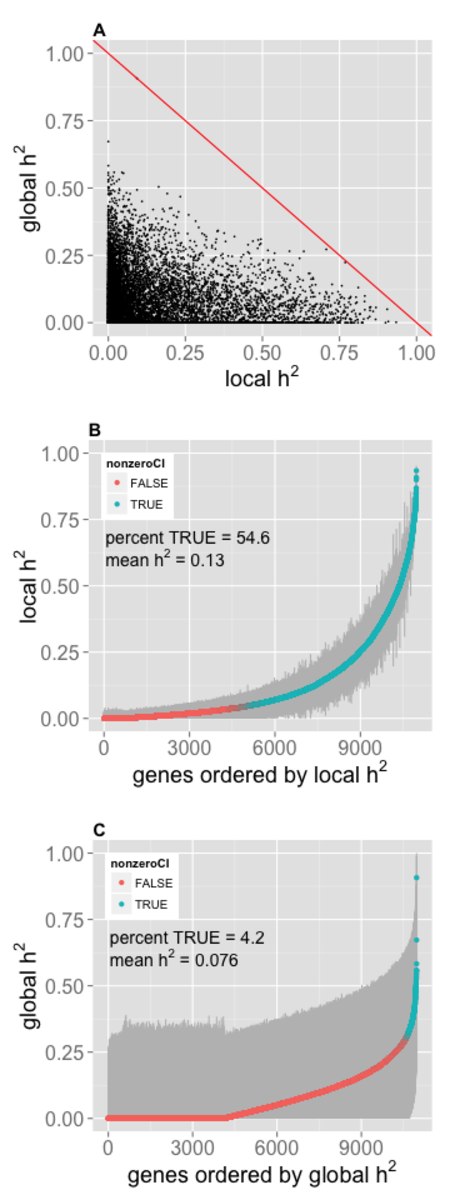
\includegraphics{GenArch_manuscript_files/figure-latex/jointH2-1.pdf}
\caption{DGN whole blood expression joint heritability
(h\textsuperscript{2}). Local (SNPs within 1 Mb of each gene) and global
(SNPs that are eQTLs in the Framingham Heart Study on other chromosomes
{[}FDR \textless{} 0.05{]}) h\textsuperscript{2} for gene expression
were jointly estimated. (\textbf{A}) Global h\textsuperscript{2}
compared to local h\textsuperscript{2} per gene. (\textbf{B}) Local and
(\textbf{C}) global gene expression h\textsuperscript{2} estimates
ordered by increasing h\textsuperscript{2}. The 95\% confidence interval
(CI) of each h\textsuperscript{2} estimate is in gray and genes with a
lower bound greater than zero are in blue.}
\end{figure}

\begin{figure}[htbp]
\centering
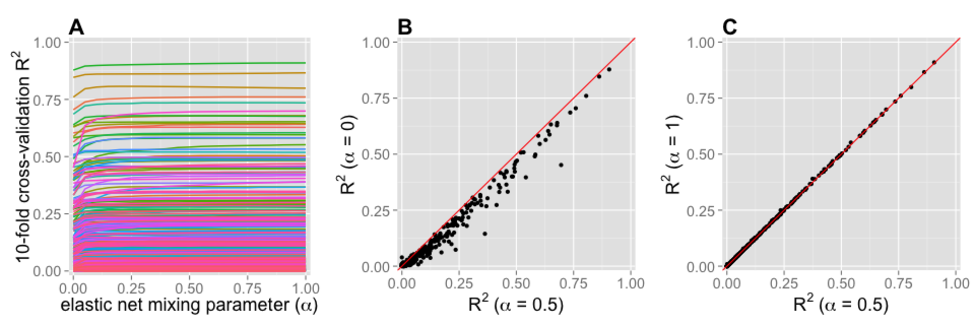
\includegraphics{GenArch_manuscript_files/figure-latex/EN-1.pdf}
\caption{Cross-validated predictive performance across the elastic net.
(\textbf{A}) 10-fold cross-validated R\textsuperscript{2} of predicted
vs.~observed expression in DGN whole blood compared to a range of
elastic net mixing parameters ($\alpha$) for 341 genes on chromosome 22.
(\textbf{B}) Predictive R\textsuperscript{2} for $\alpha = 0$ (ridge
regression) compared to $\alpha = 0.5$. (\textbf{C}) Predictive
R\textsuperscript{2} for $\alpha = 1$ (lasso) compared to
$\alpha = 0.5$.}
\end{figure}

\begin{figure}[htbp]
\centering
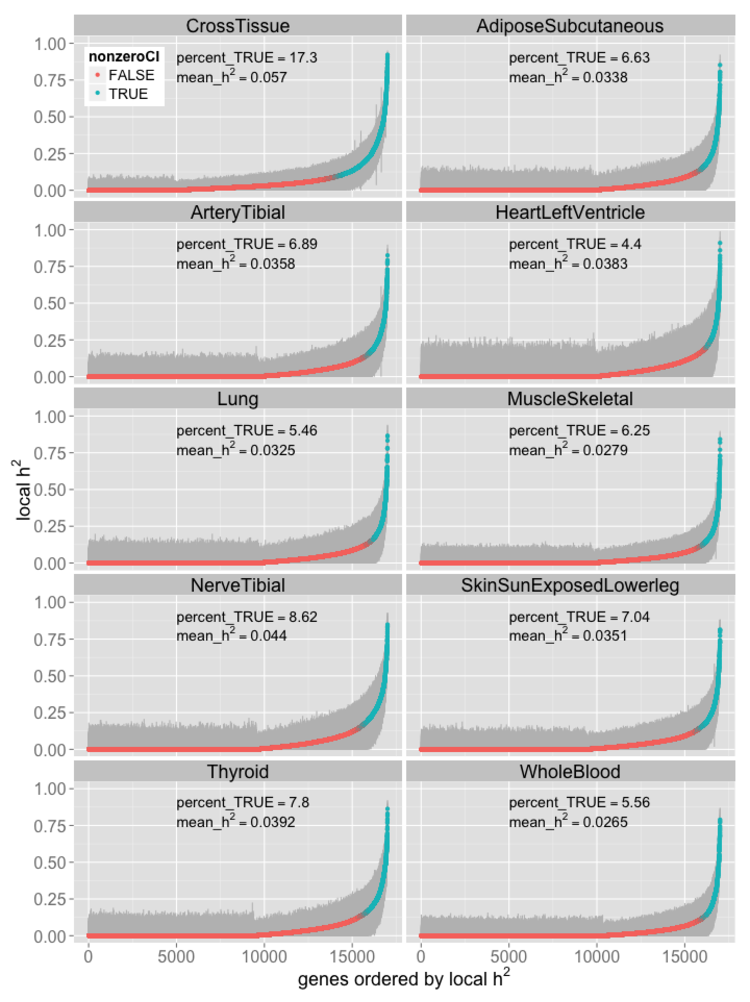
\includegraphics{GenArch_manuscript_files/figure-latex/otdTWh2-1.pdf}
\caption{Cross-tissue heritability (h\textsuperscript{2}) compared to
tissue-wide h\textsuperscript{2}. Cross-tissue local
h\textsuperscript{2} is estimated using the cross-tissue component
(random effects) of the mixed effects model for gene expression and SNPs
within 1 Mb of each gene. Tissue-wide local h\textsuperscript{2} is
estimated using the measured gene expression for each respective tissue
and SNPs within 1 Mb of each gene.}
\end{figure}

\begin{figure}[htbp]
\centering
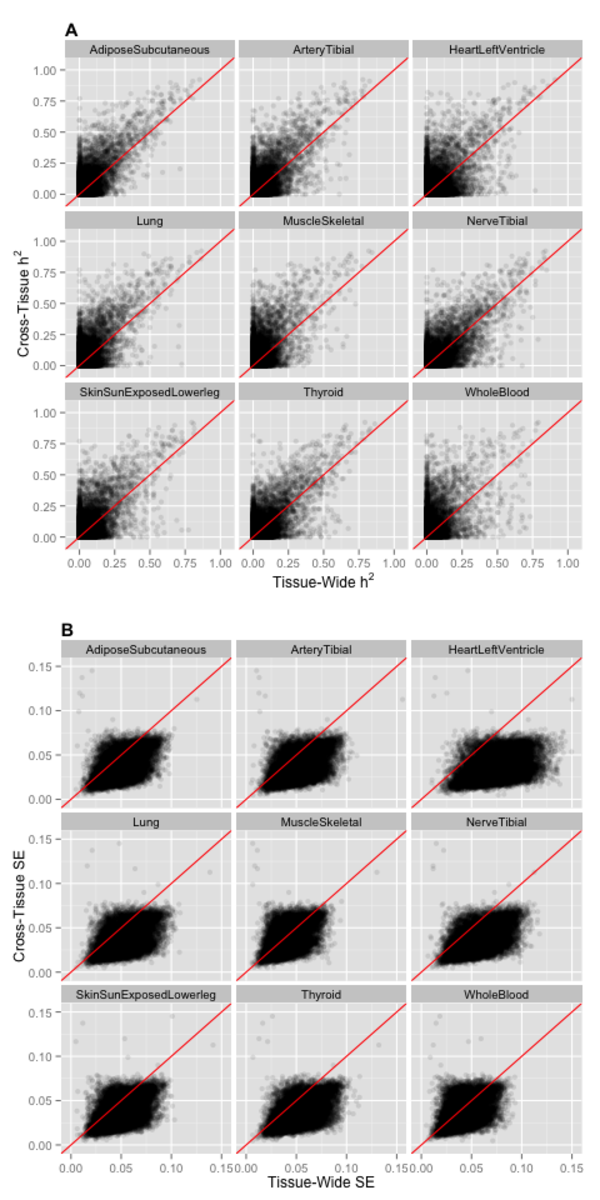
\includegraphics{GenArch_manuscript_files/figure-latex/otdTWh2SE-1.pdf}
\caption{Cross-tissue and tissue-wide comparison of heritability
(h\textsuperscript{2}, \textbf{A}) and standard error (SE, \textbf{B}).
Cross-tissue local h\textsuperscript{2} is estimated using the
cross-tissue component (random effects) of the mixed effects model for
gene expression and SNPs within 1 Mb of each gene. Tissue-wide local
h\textsuperscript{2} is estimated using the measured gene expression for
each respective tissue and SNPs within 1 Mb of each gene.}
\end{figure}

\section{Supplemental Figures}\label{supplemental-figures}

\begin{figure}[htbp]
\centering
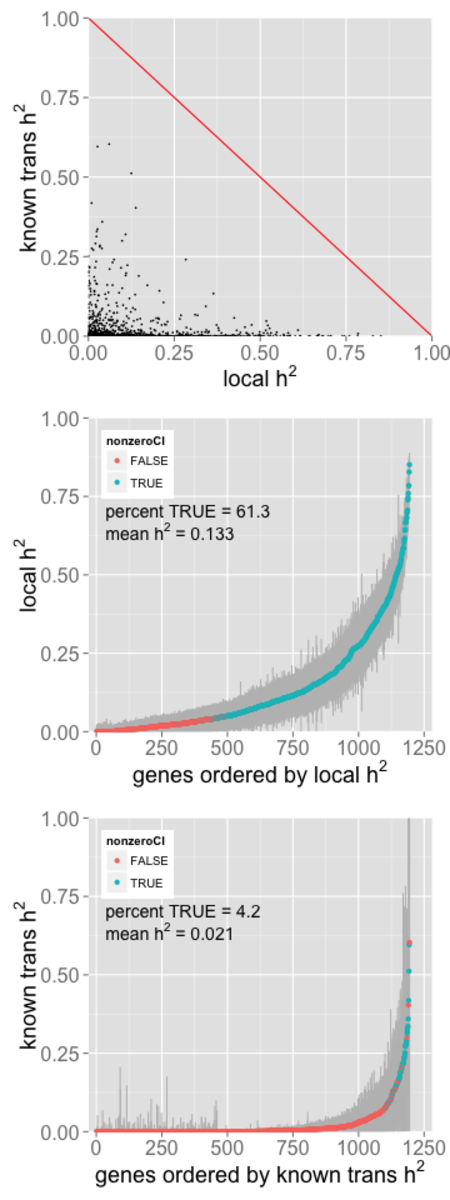
\includegraphics{GenArch_manuscript_files/figure-latex/transH2-1.pdf}
\caption{DGN whole blood expression joint heritability
(h\textsuperscript{2}) with known trans-eQTLs. Local (SNPs within 1 Mb
of each gene) and known trans (SNPs that are trans-eQTLs in the
Framingham Heart Study for each gene {[}FDR \textless{} 0.05{]})
h\textsuperscript{2} for gene expression were jointly estimated.
(\textbf{A}) Known trans h\textsuperscript{2} compared to local
h\textsuperscript{2} per gene. (\textbf{B}) Local and (\textbf{C}) known
trans gene expression h\textsuperscript{2} estimates ordered by
increasing h\textsuperscript{2}. The 95\% confidence interval (CI) of
each h\textsuperscript{2} estimate is in gray and genes with a lower
bound greater than zero are in blue.}
\end{figure}

\begin{figure}[htbp]
\centering
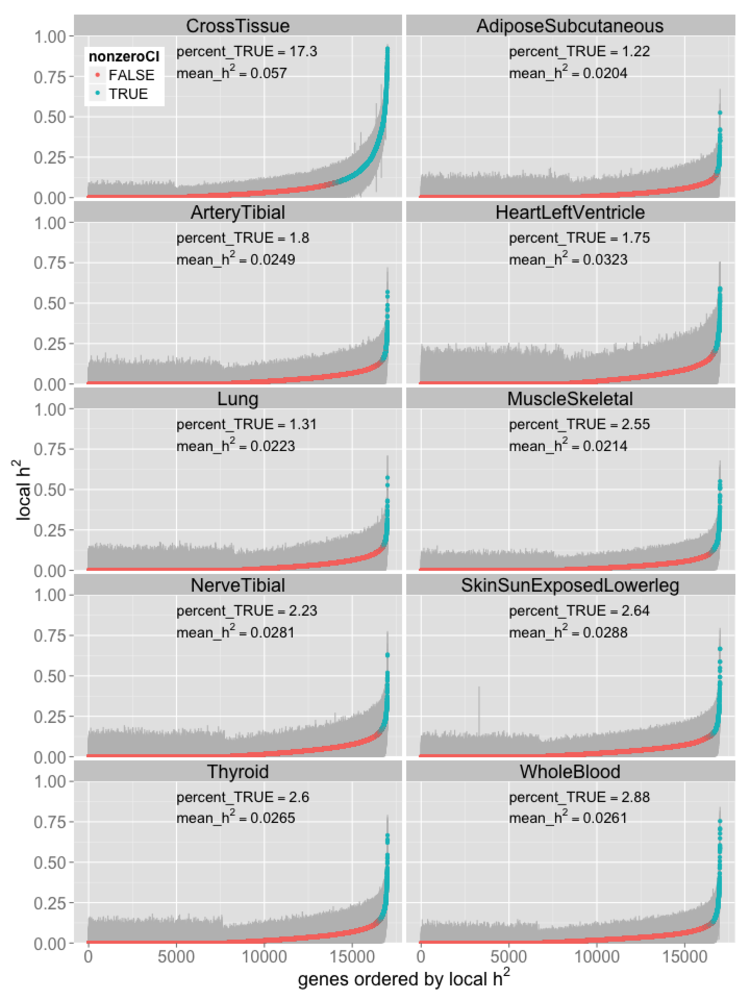
\includegraphics{GenArch_manuscript_files/figure-latex/otdTSh2-1.pdf}
\caption{Cross-tissue heritability (h\textsuperscript{2}) compared to
tissue-specific h\textsuperscript{2}. Cross-tissue local
h\textsuperscript{2} is estimated using the cross-tissue component
(random effects) of the mixed effects model for gene expression and SNPs
within 1 Mb of each gene. Tissue-specifc local h\textsuperscript{2} is
estimated using the tissue-specific component (residuals) of the mixed
effects model for gene expression for each respective tissue and SNPs
within 1 Mb of each gene.}
\end{figure}

\begin{figure}[htbp]
\centering
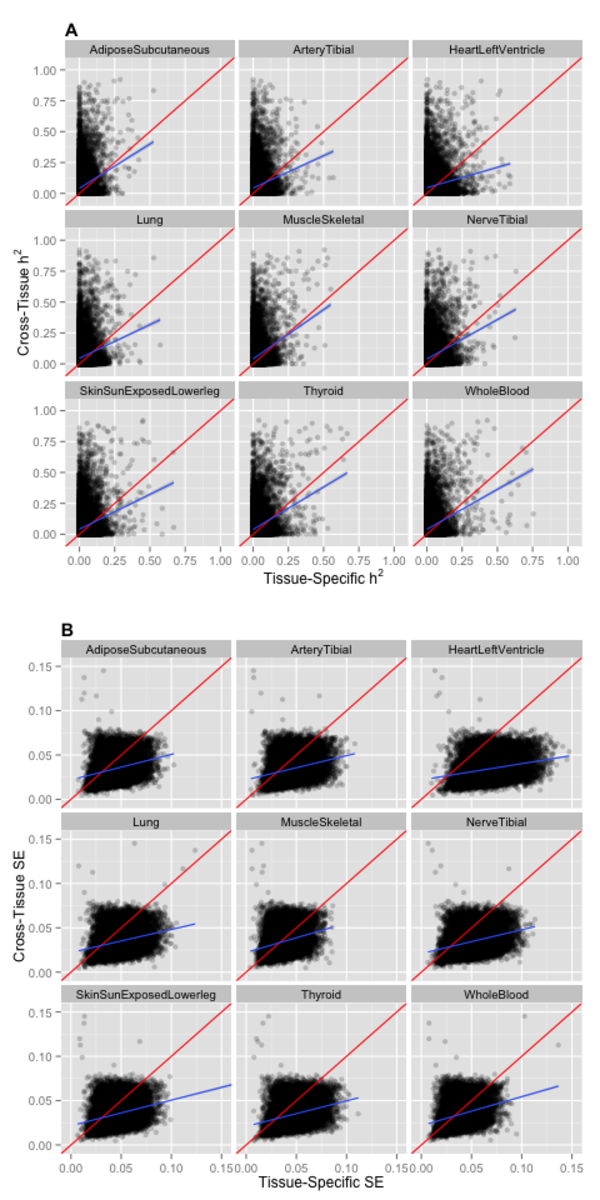
\includegraphics{GenArch_manuscript_files/figure-latex/otdTSh2SE-1.pdf}
\caption{Cross-tissue and tissue-specific comparison of heritability
(h\textsuperscript{2}, \textbf{A}) and standard error (SE, \textbf{B})
estimation. Cross-tissue local h\textsuperscript{2} is estimated using
the cross-tissue component (random effects) of the mixed effects model
for gene expression and SNPs within 1 Mb of each gene. Tissue-specifc
local h\textsuperscript{2} is estimated using the tissue-specific
component (residuals) of the mixed effects model for gene expression for
each respective tissue and SNPs within 1 Mb of each gene.}
\end{figure}

\section*{References}\label{references}
\addcontentsline{toc}{section}{References}

1. Battle A, Mostafavi S, Zhu X, Potash JB, Weissman MM, McCormick C, et
al. Characterizing the genetic basis of transcriptome diversity through
RNA-sequencing of 922 individuals. Genome Research. Cold Spring Harbor
Laboratory Press; 2013;24: 14--24.
doi:\href{http://dx.doi.org/10.1101/gr.155192.113}{10.1101/gr.155192.113}

2. Yang J, Lee SH, Goddard ME, Visscher PM. GCTA: A tool for genome-wide
complex trait analysis. The American Journal of Human Genetics. Elsevier
BV; 2011;88: 76--82.
doi:\href{http://dx.doi.org/10.1016/j.ajhg.2010.11.011}{10.1016/j.ajhg.2010.11.011}

3. Zhang X, Joehanes R, Chen BH, Huan T, Ying S, Munson PJ, et al.
Identification of common genetic variants controlling transcript isoform
variation in human whole blood. Nat Genet. Nature Publishing Group;
2015;47: 345--352.
doi:\href{http://dx.doi.org/10.1038/ng.3220}{10.1038/ng.3220}

4. Halpern BS, Regan HM, Possingham HP, McCarthy MA. Accounting for
uncertainty in marine reserve design. Ecol Letters. Wiley-Blackwell;
2006;9: 2--11.
doi:\href{http://dx.doi.org/10.1111/j.1461-0248.2005.00827.x}{10.1111/j.1461-0248.2005.00827.x}

5. Keil P, Belmaker J, Wilson AM, Unitt P, Jetz W. Downscaling of
species distribution models: a hierarchical approach. Freckleton R,
editor. Methods Ecol Evol. Wiley-Blackwell; 2012;4: 82--94.
doi:\href{http://dx.doi.org/10.1111/j.2041-210x.2012.00264.x}{10.1111/j.2041-210x.2012.00264.x}

6. R Core Team. R: A language and environment for statistical computing
{[}Internet{]}. Vienna, Austria: R Foundation for Statistical Computing;
2014. Available: \url{http://www.R-project.org/}

7. Boettiger C. knitcitations: Citations for knitr markdown files
{[}Internet{]}. 2014. Available:
\url{http://CRAN.R-project.org/package=knitcitations}

\end{document}
